\chapter{Detailed description of the subject of analysis}

\section{The market and the observation point}
The public website \url{https://metin2alerts.com/store/} provides a practical observation point of the in-game market: it displays items listed for sale by players, along with their prices and detailed properties.
From an analytical perspective, this site acts as a \textbf{public market monitor}, allowing the observation of supply, demand, and pricing dynamics without requiring direct access to the game servers.
Figure~\ref{fig:metin2alerts_market} showcases a screenshot of the platform, illustrating how market data is publicly accessible and structured.
\begin{figure}[H]
    \centering
    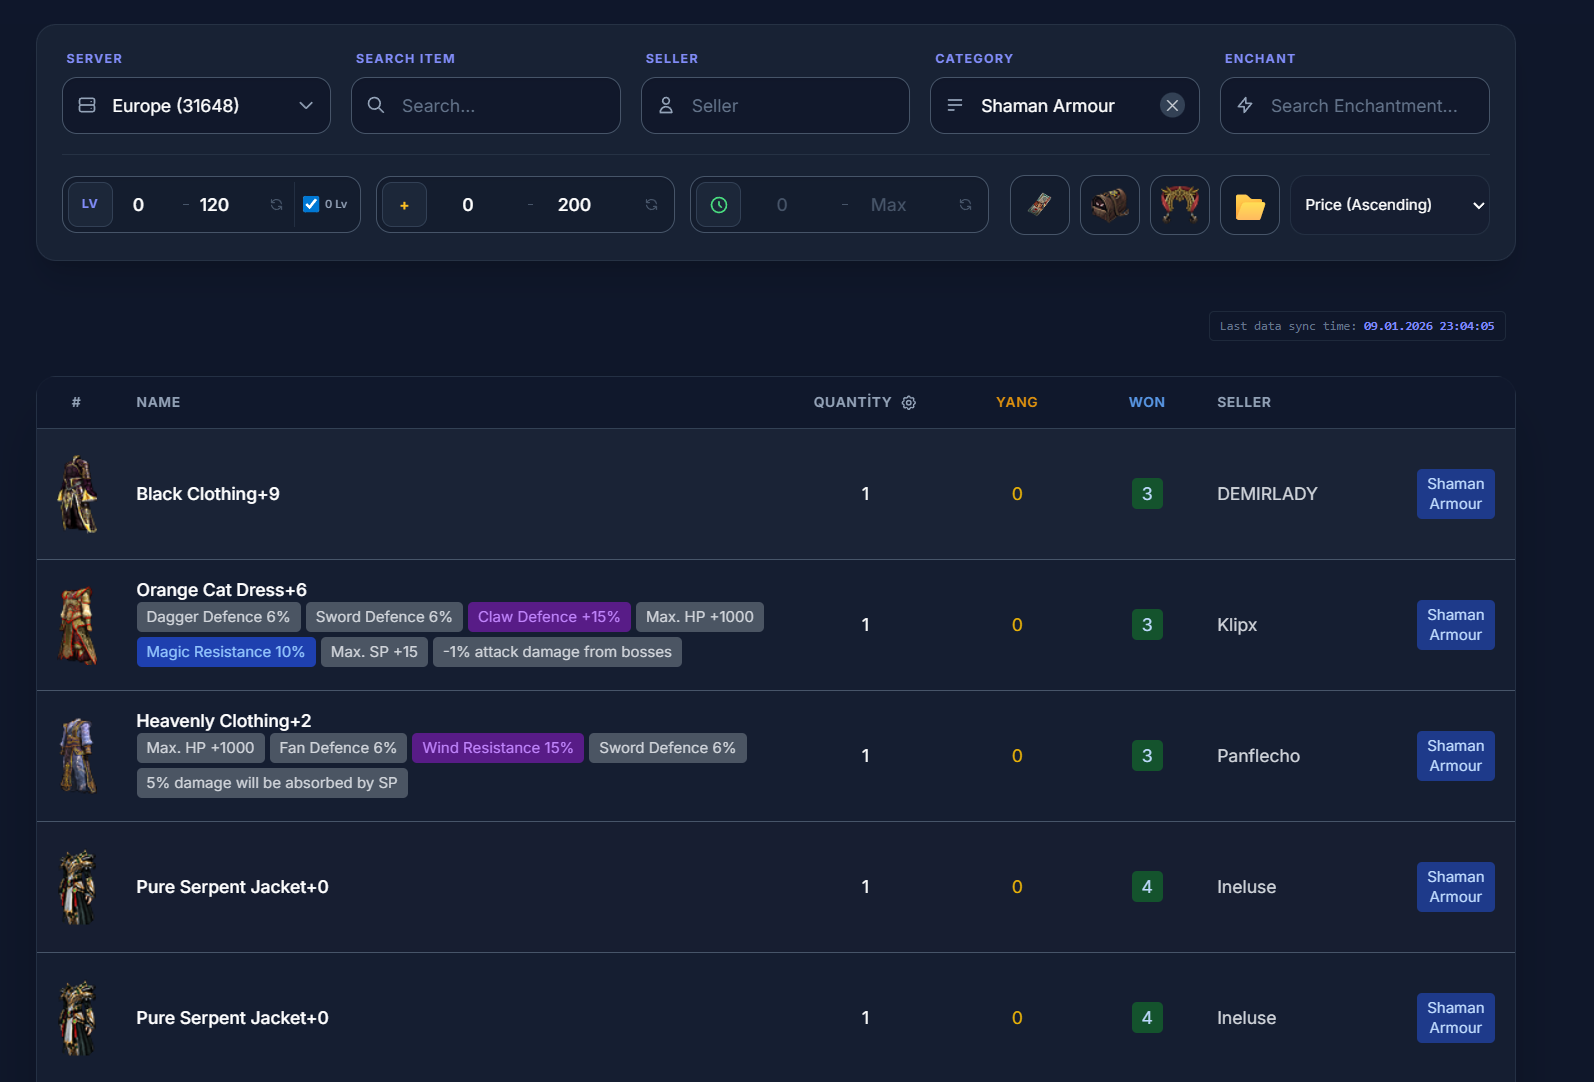
\includegraphics[width=0.7\linewidth]{metin2alerts_market.png}
    \caption{Screenshot of the Metin2Alerts marketplace showing listed items, prices, and item attributes}
    \label{fig:metin2alerts_market}
\end{figure}


\subsection{Currency model (Yang and Won)}
Prices are expressed using two in-game currencies:
\begin{itemize}
  \item \textbf{Yang}: the most common currency used for everyday trades (``small change'').
  \item \textbf{Won}: higher denomination currency used for expensive items (``big bills'').
\end{itemize}
In the warehouse, both are stored so analyses can handle cheap and expensive items consistently.

\subsection{Objects of analysis and granularity}
The primary object of analysis is a \textbf{market listing snapshot}. A snapshot represents the market state at a given capture time.
For decision support, we analyze the market at multiple granularities:
\begin{itemize}
  \item \textbf{Listing level}: seller, server, prices (Yang/Won), and quantity.
  \item \textbf{Item identity level}: 
  the \texttt{vnum} item identifier for grouping and trend tracking.
  \item \textbf{Item instance properties}: enhancement level, sockets, and bonus attributes that influence the price.
  \item \textbf{Time level}: daily time dimension for trends and volatility metrics.
\end{itemize}

\subsection{Key measures and KPIs}
The system targets measurable indicators needed for market decisions:
\begin{itemize}
  \item \textbf{Price statistics}: average/min/max prices per item and period.
  \item \textbf{Trend and volatility}: trend direction (up/down/stable) and volatility score.
  \item \textbf{Deal detection}: undervaluation percentage, potential profit, and confidence score.
  \item \textbf{Attribute-driven value}: rarity score and value multipliers from bonuses.
\end{itemize}

\section{Decision-making issues}
Players and traders face several recurring decision problems:
\begin{itemize}
  \item \textbf{Fair pricing}: determining whether a listed item price is normal, expensive, or a bargain.
  \item \textbf{Trend detection}: understanding if an item is going up/down over time.
  \item \textbf{Attribute impact}: quantifying how bonuses/enchantments and enhancement level affect price.
  \item \textbf{Server differences}: comparing the same item across different servers.
\end{itemize}

\section{Stakeholders}
\begin{itemize}
  \item \textbf{Casual players}: want quick guidance to avoid overpaying.
  \item \textbf{Traders}: search for undervalued listings and arbitrage opportunities.
  \item \textbf{Guild leaders}: plan equipment upgrades and budget planning for members.
  \item \textbf{Market analysts}: study the economy dynamics and item liquidity.
\end{itemize}

\begin{questionbox}
\begin{enumerate}
  \item What are the \textbf{top most expensive items} on a given server in average Yang price?
  \item For a given item (\texttt{vnum}), what is the \textbf{price evolution over time}?
  \item Which listings look \textbf{undervalued} compared to an estimated fair value?
  \item How do \textbf{bonuses/enchantments} and \textbf{enhancement level} influence price?
  \item How do prices differ between \textbf{Server 502} and \textbf{Server 71}?
\end{enumerate}
\end{questionbox}

